%adobe reader fix
\pdfminorversion=4

\documentclass[final,12pt]{beamer}

%set image/logo options
% Rice
\def\RightLogoWidth{0.18}
\def\RightLogoPaddingTop{0.25cm}
\def\RightLogoPaddingBottom{0.5cm}
\def\RightLogo{../../logos/RiceLogo_TMCMYK300DPI.jpg}
% SHINE
\def\LeftLogoWidth{0.17}
\def\LeftLogoPaddingTop{0.5cm}
\def\LeftLogoPaddingBottom{0.5cm}
\def\LeftLogo{../../logos/shine-logo.png}
% SunPy
\def\AnotherLeftLogoWidth{0.06}
\def\AnotherLeftLogoPaddingTop{0.25cm}
\def\AnotherLeftLogoPaddingBottom{0.25cm}
\def\AnotherLeftLogo{../../logos/sunpy_powered_logo.png}
% Title and author(s) block
\def\TitleWidth{0.55}
% GitHub
\def\GitHubLogoWidth{0.014\paperwidth}
\def\GitHubLogo{../../logos/GitHub-Mark-120px-plus.png}
\def\GitHubUser{wtbarnes}
% Affiliation in footer
\def\AffiliationFooter{Department of Physics and Astronomy - Rice University - Houston, TX USA}
% Email
\def\EmailAddressFooter{will.t.barnes@rice.edu}

%set theme
\mode<presentation>
{
\usetheme{I6dv_custom}
}
\setbeamertemplate{caption}[numbered]
%\usefonttheme[onlymath]{serif}

%Include packages
\usepackage{soul,color,verbatim}
\usepackage{amsmath,amsthm,amssymb}
\usepackage{graphicx}
\usepackage{epstopdf}
\usepackage[numbers]{natbib}
\usepackage{multicol}
\usepackage[english]{babel}
%\usepackage[latin1]{inputenc}
\usepackage{tikz}
%setup beamerposter package, use 3-by-4 feet
\usepackage[orientation=portrait,size=custom,width=91.44,height=121.92,scale=1.0]{beamer/beamerposter/beamerposter}

%tikz configuration

%custom commands go here
\newcommand{\ang}{\AA~} %alias angstrom
\DeclareMathOperator*{\argmax}{arg\,max} % in your preamble
\setbeamerfont{caption}{size=\footnotesize} %make caption size small

%Set author and title
\title[]{Using Synthetic and Observed Timelags to Constrain Nanoflare\\ Heating Properties in Active Region Cores}
\author[Barnes, Bradshaw, \& Viall]{Will T. Barnes\inst{1}, Stephen J. Bradshaw\inst{1}, \& Nicholeen Viall\inst{2}}
\institute[]{\inst{1} Department of Physics and Astronomy, Rice University \inst{2} NASA Goddard Space Flight Center}
\date{30 July-3 August, 2018}

%start poster
%everything goes in one frame
\begin{document}
\begin{frame}
  %start columns environment to slice up the page horizontally
  \begin{columns}[T]
  \hfill
  %%
  %%first column
  \begin{column}{0.49\linewidth}
    %
    %introduction
    \begin{block}{Introduction}
    \vspace{-2ex}
    \begin{itemize}
      \item Long-standing debate around whether active regions are heated \alert{steadily or impulsively}
      \item Fundamental question: \alert{what is the frequency at which individual loops in active regions are reenergized?}
      \item Observations often interpreted in context of nanoflare heating \citep[e.g.][]{brosius_pervasive_2014,ishikawa_detection_2017}, though steady heating also possible \citep{winebarger_investigation_2016}
      \item Two primary queestions: \alert{1.How do observable signatures vary with heating frequency?} and \alert{2. Can we use synthetic observables together with real data to constrain properties of the heating?}
      \item Timelags between AIA channel pairs \citep{viall_evidence_2012,viall_survey_2017} provide a powerful diagnostic for cooling patterns 
      \item Explore a range of heating frequencies and systematically assess model viability based on detailed comparisons to data---\alert{a successful model must be consistent with all observables}
      \item Forward model active region emission using ensemble of field-aligned hydrodynamic models and detailed atomic physics
    \end{itemize}
    \vspace{-1ex}
    \end{block}
    %
    % forward modeling
    %% Describe synthesizAR code, maybe a diagram?
    \begin{block}{Pipeline for Forward Modeling Emission from Active Region Cores}
      \vspace{-2ex}
      \begin{columns}[c]
      \begin{column}{0.33\columnwidth}
        \begin{figure}
        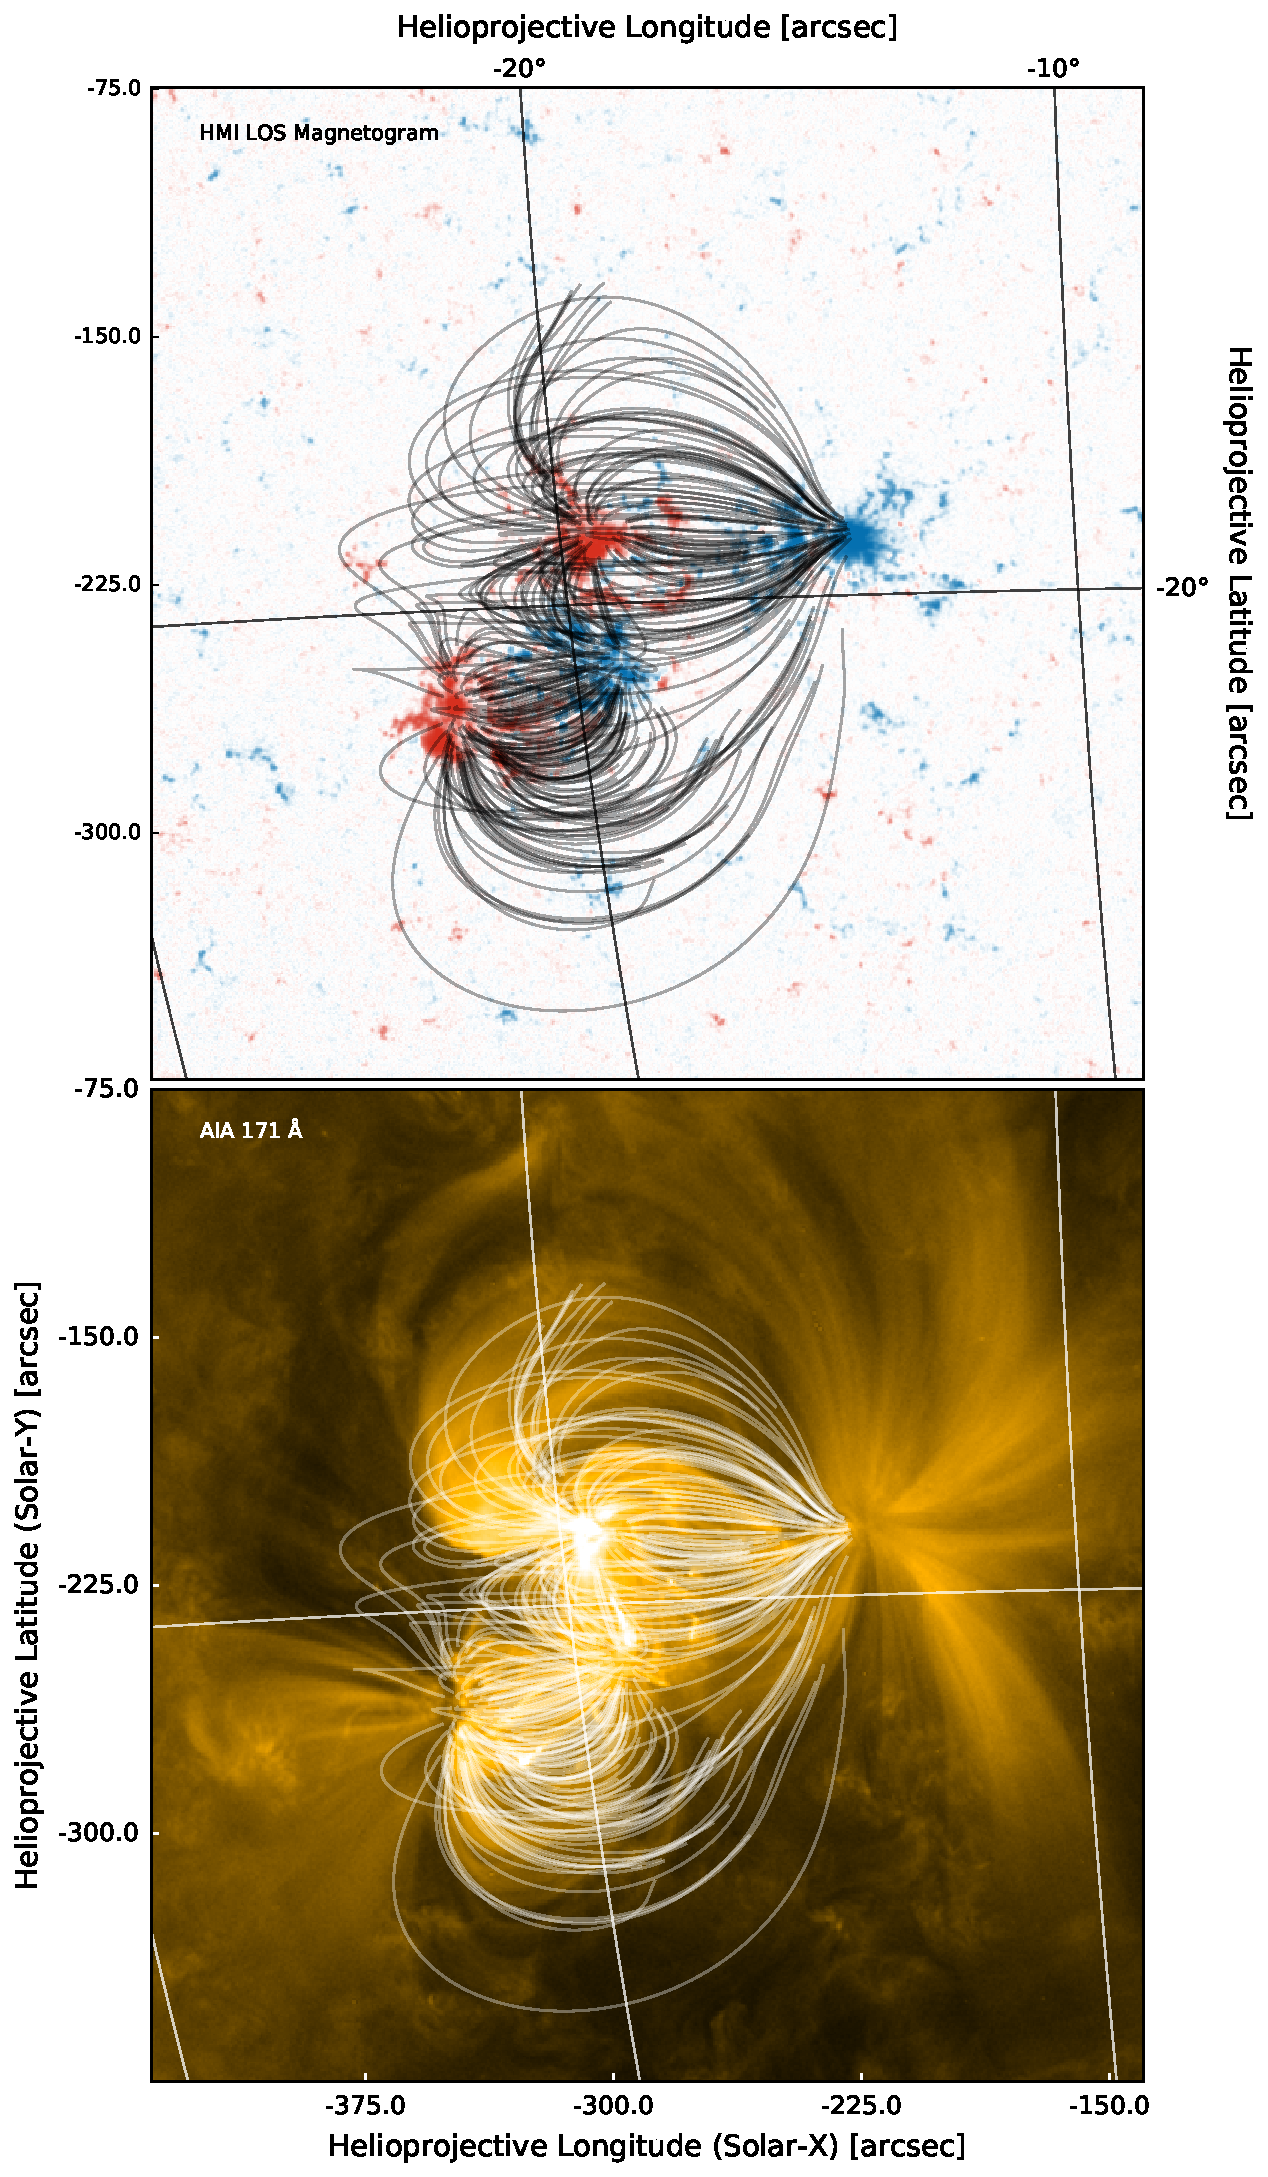
\includegraphics{../figures/hmi_plus_aia_plus_lines.pdf}
        \label{fig:hmi_plus_aia}
        \caption{HMI LOS magnetogram (\textbf{Top}) and AIA 171 \AA\,\,image (\textbf{Bottom}) of NOAA 1158 observed on 12 February 2011 with $\sim250$ fieldines overlaid from a potential field extrapolation}
        \end{figure}
      \end{column}
      \begin{column}{0.65\columnwidth}
        \begin{enumerate}
          \item Select magnetogram for the desired active region. Fig. \ref{fig:hmi_plus_aia} shows NOAA 1158 as observed by HMI and AIA. 
          \item Perform a field extrapolation to derive the three-dimensional vector field $\vec{B}$ using oblique Schmidt method \citep{schmidt_observable_1964}
          \item Trace 5000 fieldlines through extrapolated field, including only closed fieldlines  with loop lengths in the range $20<L<300$ Mm.
          \item For each fieldline, run a field-aligned hydrodynamic model. In this case, we'll use the two-fluid ebtel++ model described in \citet{barnes_inference_2016} and compute $3\times10^4$ s of evolution
          \item Using $T_e$ and $n_e$ from hydrodynamic model, calculate emissivity for each selected transition $\lambda_{ij}$ of element $X$ and charge state $k$,
            \begin{equation*}
              P_{ij}(X,k) = \frac{n_h}{n_e}\text{Ab}(X)f_{X,k}(T_e)N_j(n_e,T_e)A_{ij}\Delta E_{ij}n_e
            \end{equation*}
            \begin{itemize}
              \item $\text{Ab}(X),N_j,A_{ij},\Delta E_{ij}$ all computed or read from CHIANTI v8.0.6 \citep{young_chianti_2016,dere_chianti_1997}
              \item Coronal abundances from \citet{feldman_potential_1992}
              \item Include all transitions of all ions from calcium, iron, magnesium, nickel, oxygen, silicon, and sulfur
              \item $f_{X,k}$ calculation includes effects due to nonequilibrium ionization using methods of \citep{bradshaw_numerical_2009}
              \item $T_e,n_e$ functions of $h$, the distance along the LOS which intersects \textit{many} loops
            \end{itemize}
          \item Integrate the emissivity along the LOS for each transition and convolve with the instrument response,
            \begin{equation*}
              I_c = \frac{1}{4\pi}\int_{\text{LOS}}\text{d}h\left(\sum_{\{ij\}}P_{ij}R_c(\lambda_{ij})\right)
            \end{equation*}
            where $R_c$ is the AIA wavelength response for channel $c$ and $I_c$ is the resulting channel intensity
          \item Convolve with the point spread function of the instrument.
        \end{enumerate}
      \end{column}
      \end{columns}
    \end{block}
    %
    % Heating model
    %% Show tN distributions
    \begin{block}{Heating Model: Impulsive Heating over a Range of Frequencies}
      \vspace{-2ex}
      \begin{columns}[c]
        \begin{column}{0.5\columnwidth}
          \begin{itemize}
            \item Parameterize heating in terms of \alert{discrete triangular pulses of duration 200 s} occurring on individual strands, i.e. nanoflares \citep{parker_nanoflares_1988}
            \item Define the heating frequency in terms of the loop cooling time $\tau_{cool}$ such that,
            \begin{equation*}
              \varepsilon = \frac{\langle t_{wait}\rangle}{\tau_{cool}}\begin{cases} 
                < 1, & \text{high frequency}, \\
                \sim1, & \text{intermediate frequency}, \\
                >1, & \text{low frequency}
             \end{cases}
            \end{equation*}
            where $t_{wait}$ is the time between successive events on a given strand
            \item Choose event energy $E_i$ from power-law distribution $P(E_0,(\epsilon B)^2/8\pi,\alpha=-2.5)$
            \item Waiting time prior to each event chosen such that $t_{wait}\propto E_i$ following model of \citet{cargill_active_2014}---the longer the field is stressed, the greater the energy release
            \item Constrain the total flux into the AR to be $\approx10^7$ erg cm$^{-2}$ s$^{-1}$ according to observations by \citet{withbroe_mass_1977}
            \item Include two additional control models:
            \begin{itemize}
              \item ``Cooling''---Each strand heated by single pulse at $t=0$ s with energy $(\epsilon B)^2/8\pi$
              \item ``Random''---Each strand heated by single pulse at some random time in $0<t<3\times10^4$ s with energy $(\epsilon B)^2/8\pi$
            \end{itemize}
          \end{itemize}
        \end{column}
        \begin{column}{0.48\columnwidth}
          \begin{figure}
            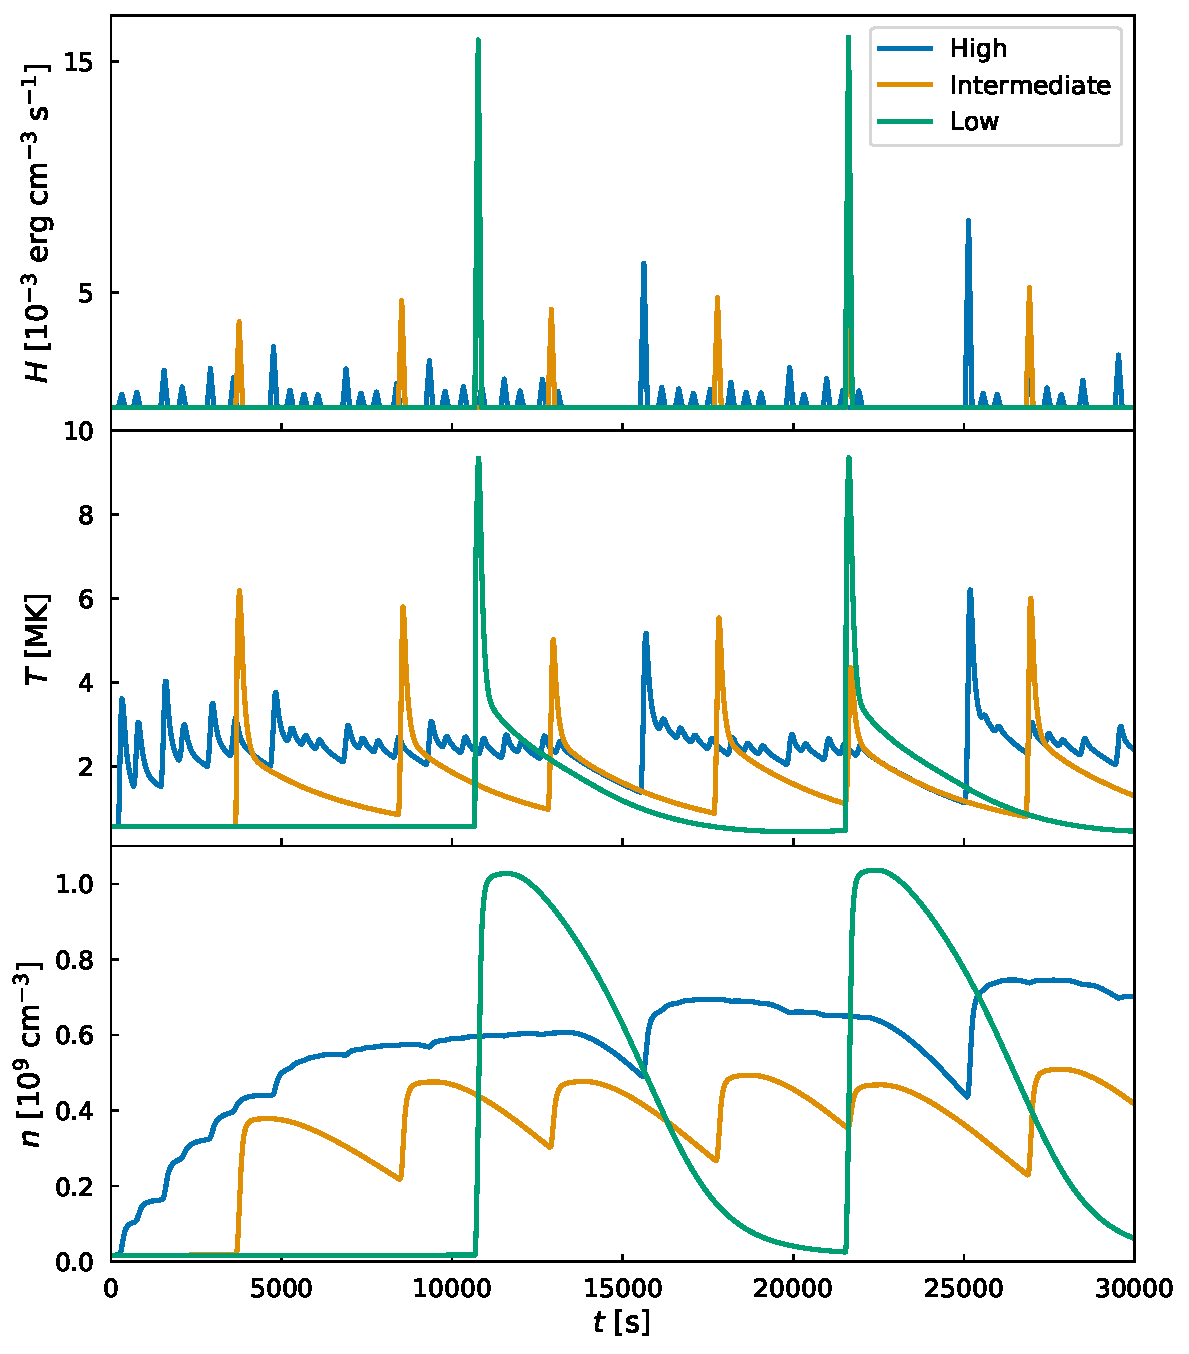
\includegraphics{../figures/hydro_profiles}
            \label{fig:hydro}
            \caption{Heating profile (\textbf{Top}), electron temperature (\textbf{Middle}), and density (\textbf{Bottom}) for each heating frequency for a single loop in the active region.}
          \end{figure}
        \end{column}
      \end{columns}
      \vspace{-1ex}
    \end{block}
    %
    % aia intensity maps
    %% show aia intensity maps for a single frequency
    \begin{block}{Simulated AIA Intensities}
      \vspace{-2ex}
      \begin{figure}
      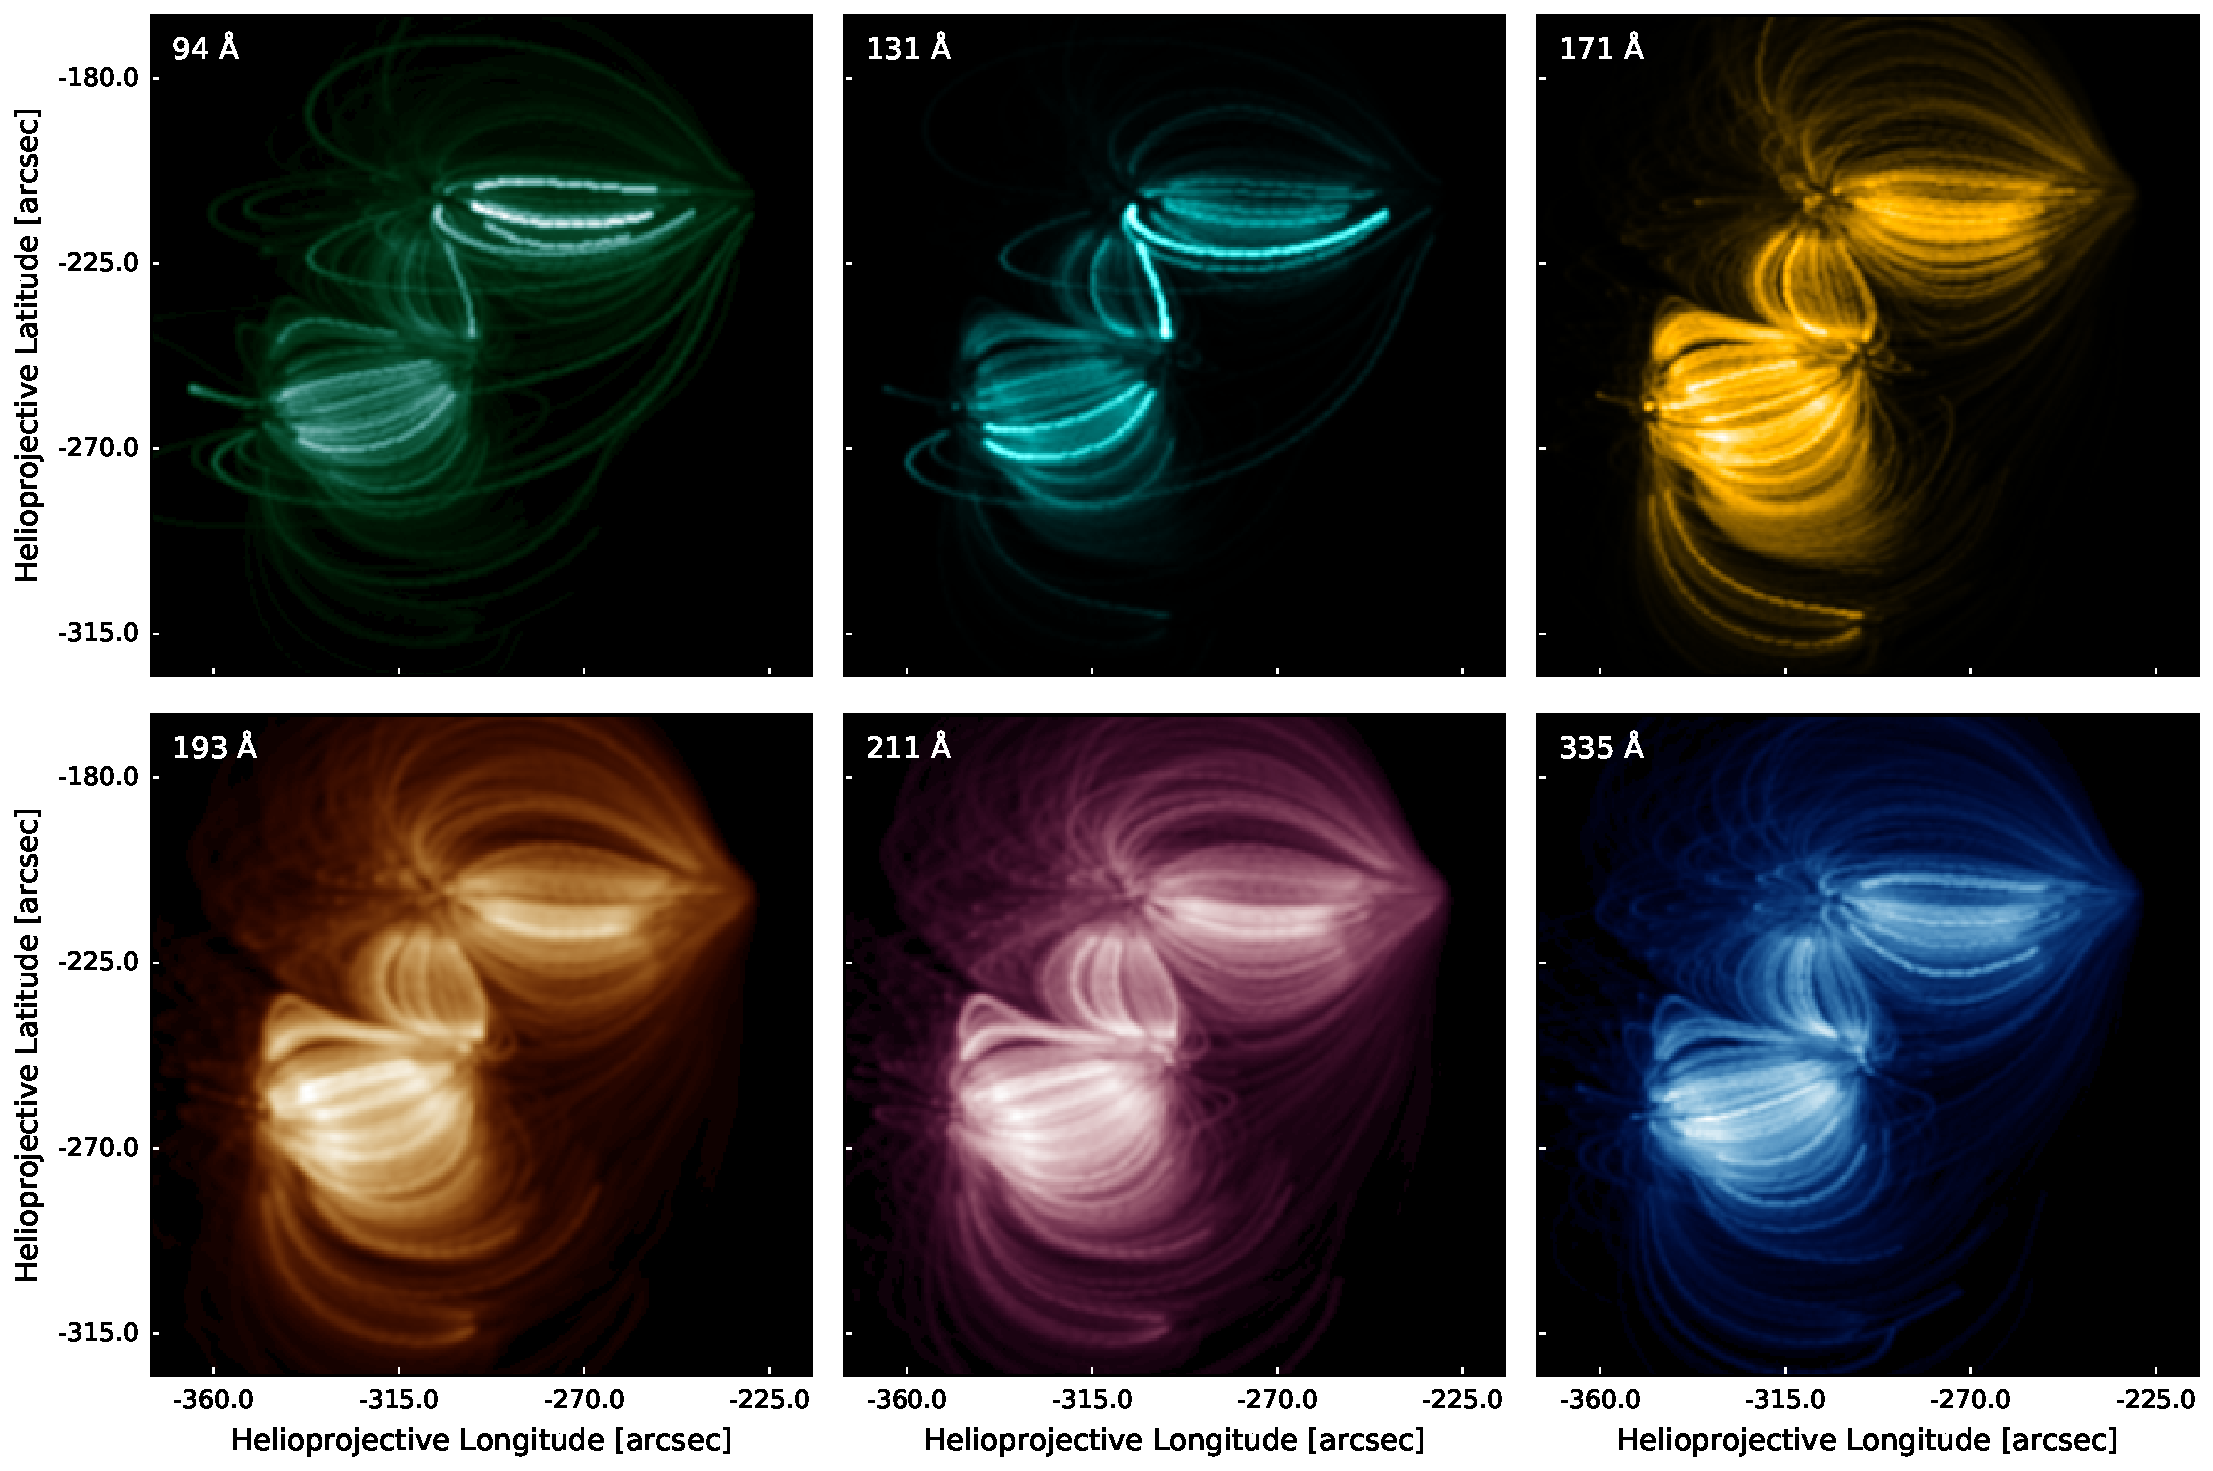
\includegraphics{../figures/aia_intensity_maps}
      \label{fig:intensity_maps}
      \caption{Snapshot of intensity at $t=2.5\times10^4$ s in three AIA channels for the intermediate frequency case}
      \end{figure}
      \vspace{-2.5ex}
    \end{block}
    %
    % timelags
    %% quantitative and qualitative explanation
    \begin{block}{Computing Timelags Between AIA Channel Pairs}
      \vspace{-4ex}
      \begin{columns}[c]
        \begin{column}{0.53\columnwidth}
          \begin{figure}
            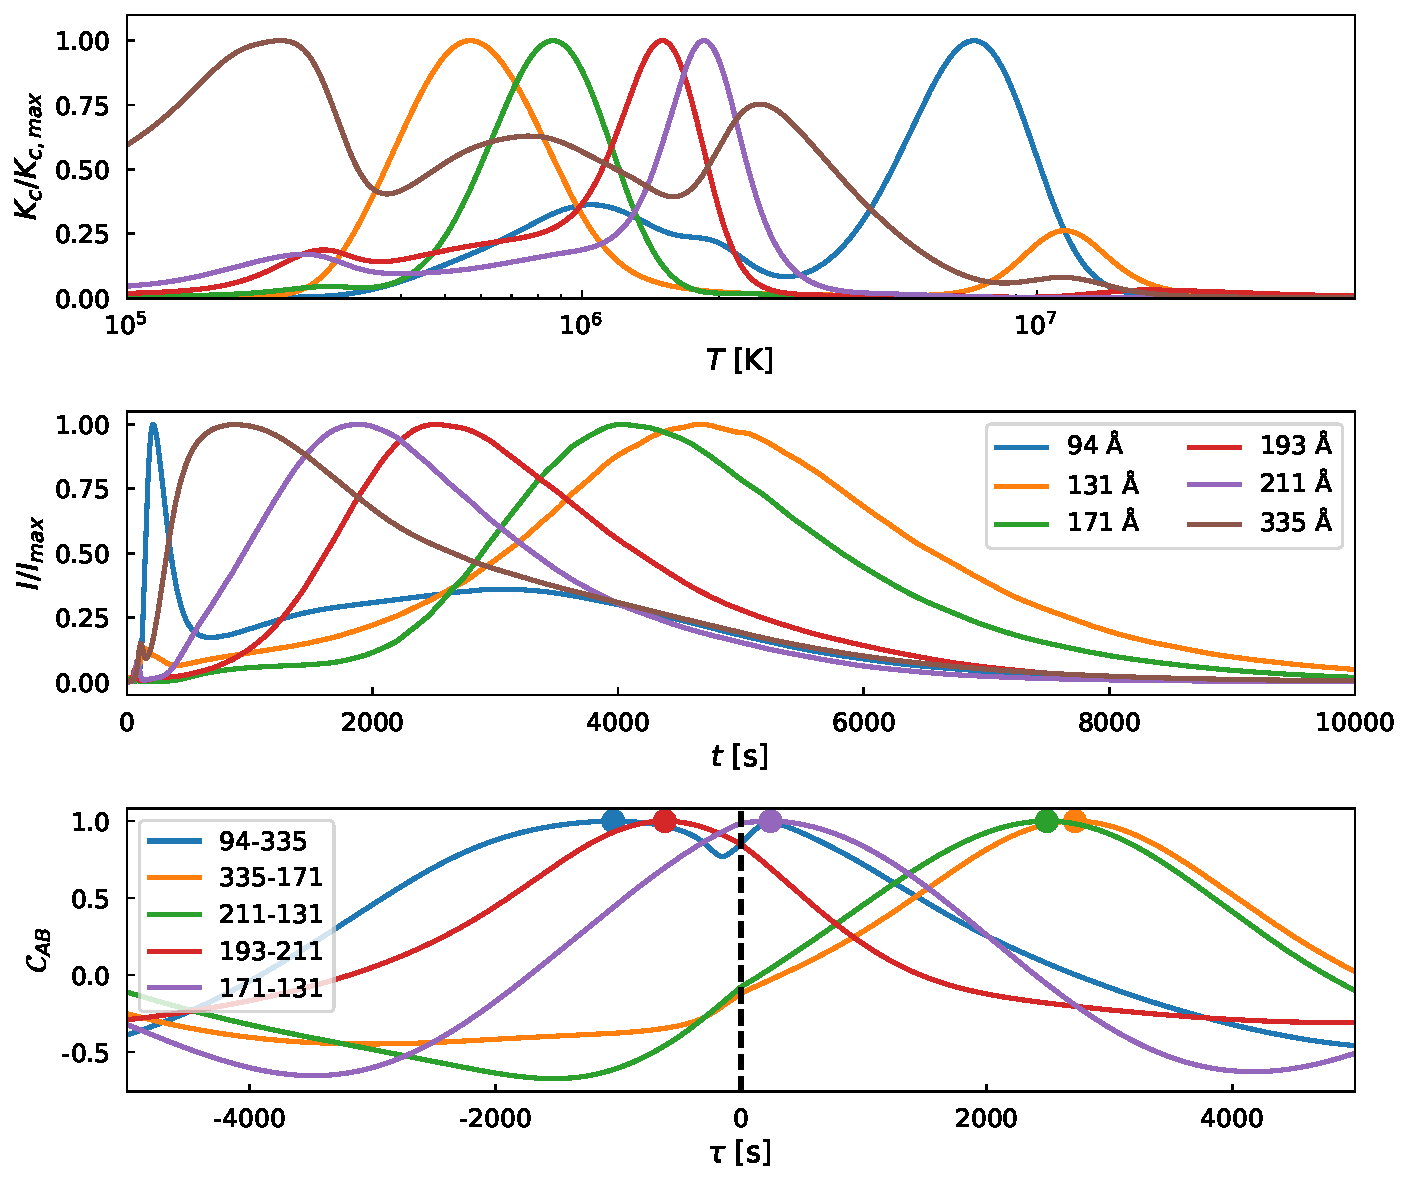
\includegraphics{../figures/timeseries_timelags_1d}
            \label{fig:timelags_1d}
            \caption{\textbf{Top:} AIA temperature response functions for 6 EUV channels; \textbf{Middle:} Normalized pixel-averaged AIA intensity for the ``cooling'' case described above; \textbf{Bottom:} Cross-correlation curves for selected channel pairs}
          \end{figure}
        \end{column}
        \begin{column}{0.45\columnwidth}
          \begin{itemize}
            \item As coronal plasma cools, the intensity peaks in successively cooler AIA passbands (see top panel of Fig. \ref{fig:timelags_1d})
            \item Understand relationship between these peaks by computing cross-correlation between channel pairs
            \item The cross-correlation between two channels $A$ and $B$ as a function of the offset $\tau$ can be expressed as,
            \begin{align*}
              \mathcal{C}_{AB}(\tau) &= I_A(t)\star I_B(t) = I_A(-t)*I_B(t),\\
              \mathcal{F}\{\mathcal{C}_{AB}(\tau)\} &= \mathcal{F}\{I_A(-t)*I_B(t)\} \\
              &= \mathcal{F}\{I_A(-t)\}\mathcal{F}\{I_B(t)\} \\
              \mathcal{C}_{AB}(\tau) &= \mathcal{F}^{-1}\{\mathcal{F}\{I_A(-t)\}\mathcal{F}\{I_B(t)\}\}
            \end{align*}
            \item Define the timelag $\tau_{AB}$ as that offset which maximizes the cross-correlation,
            \begin{align*}
              \tau_{AB} = \argmax_{\tau}(\mathcal{C}_{AB}(\tau))
            \end{align*}
            \item By convention, order hot channel first such that \alert{positive timelags indicate cooling plasma}
            \item Compute $\tau_{AB}$ in each pixel between -6 hours and +6 hours from $2\times10^4$ s of simulation time
          \end{itemize}
        \end{column}
      \end{columns}
    \end{block}
  \end{column}
  %%
%%%%%%%%%%%%%%%%%%%%%%%%%%%%%%%%%%%%%%%%%%%%%%%%%
  %%second column
  \begin{column}{0.49\linewidth}
    %
    % simulated and observed timelags
    %% maps of timelags
    \begin{block}{Simulated versus Observed Timelags}
      \vspace{-2ex}
      \begin{figure}
        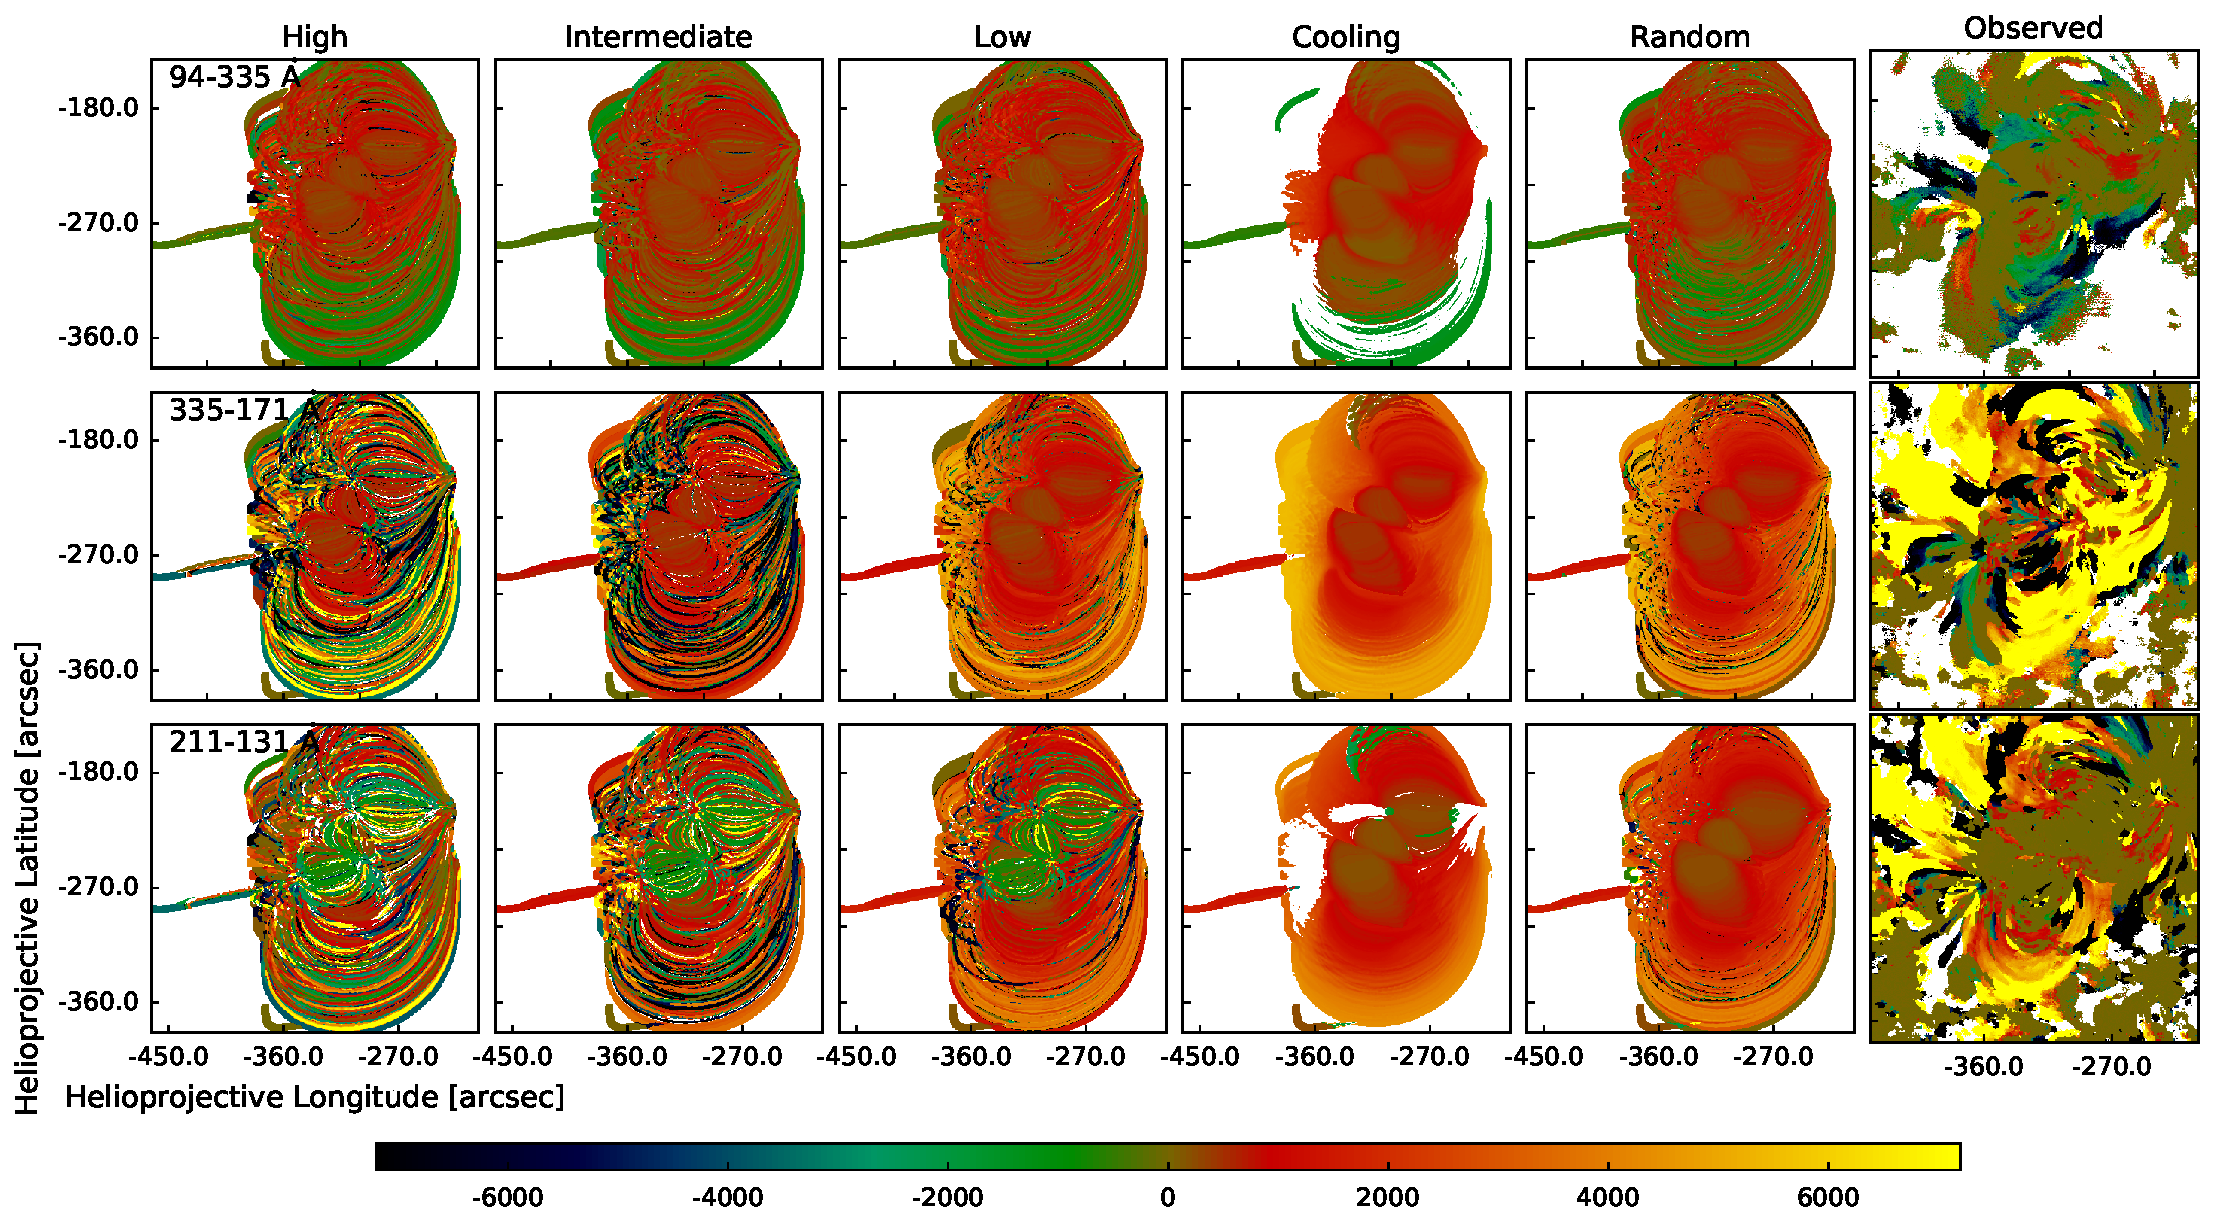
\includegraphics{../figures/timelag_maps}
        \label{fig:timelag_maps}
        \caption{$\tau_{AB}$ computed in each pixel of the AR for all five heating cases and observed intensity for three selected channel pairs. Note in particular the presence of negative timelags in the 131 \AA\,\,pair for the low, intermediate, and high frequency models and their absence in the observation}
      \end{figure}
    \end{block}
    %
    % timelag classification
    %% distribution of slopes plus overplotted results from literature
    \begin{block}{Analyzing Observed Pixels with a Random Forest Classifier}
      \begin{columns}[c]
        \begin{column}{0.35\columnwidth}
          \begin{figure}
            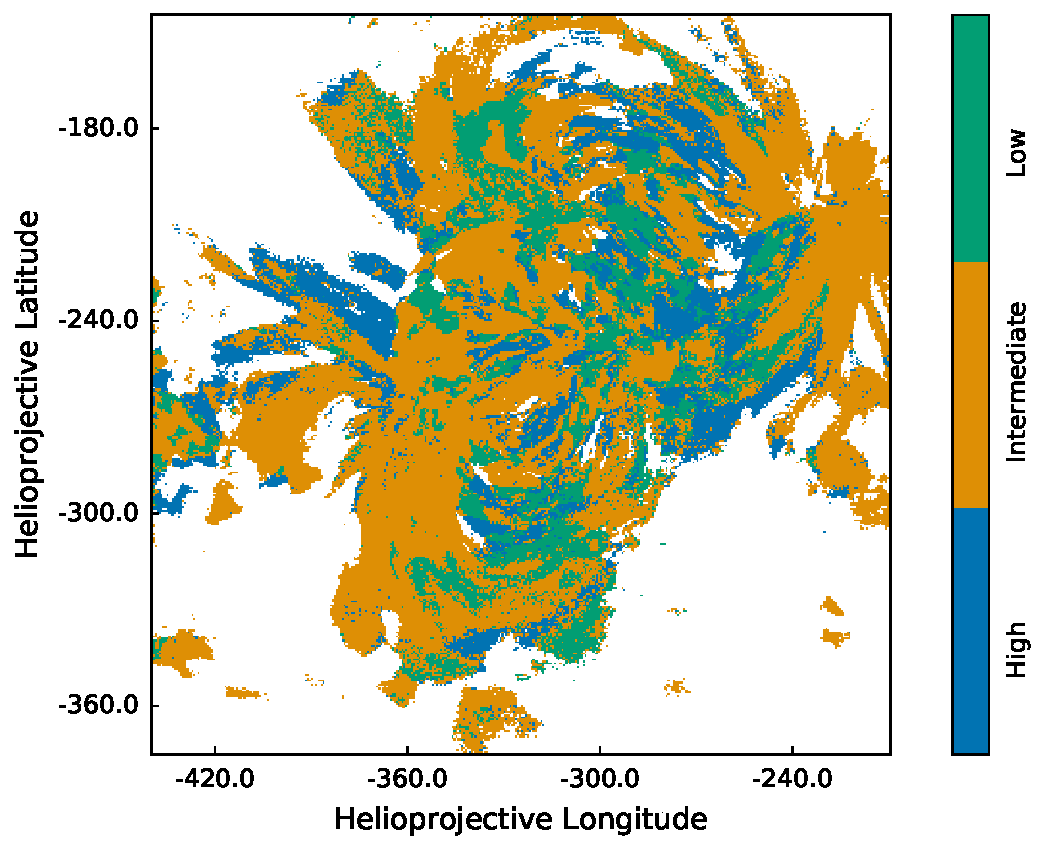
\includegraphics{../figures/class_map}
          \end{figure}
        \end{column}
        \begin{column}{0.57\columnwidth}
          \begin{itemize}
            \item Train random forest classifier on simulated timelags from all 15 channel pairs
            \item \textbf{Random Forest:} Ensemble of many decision trees trained on randomly sampled subsets of the data, designed to reduce variance (i.e. avoid overfitting)
            \item Use random forest implementation in the highly-optimized, well-documented Scikit-learn Python package \citep{pedregosa_scikit-learn_2011}
            \item Using 100 decision trees with a maximum tree depth of 25, \alert{get $\sim4\%$ misclassification error} on test dataset
            \item \alert{Systematically evaluate observed data using every dimension of simulated data}
            \item Classifier suggests \alert{dominant intermediate frequency heating}, with more low frequency heating on periphery, high frequency heating in core
          \end{itemize}
        \end{column}
      \end{columns}
      \begin{figure}
        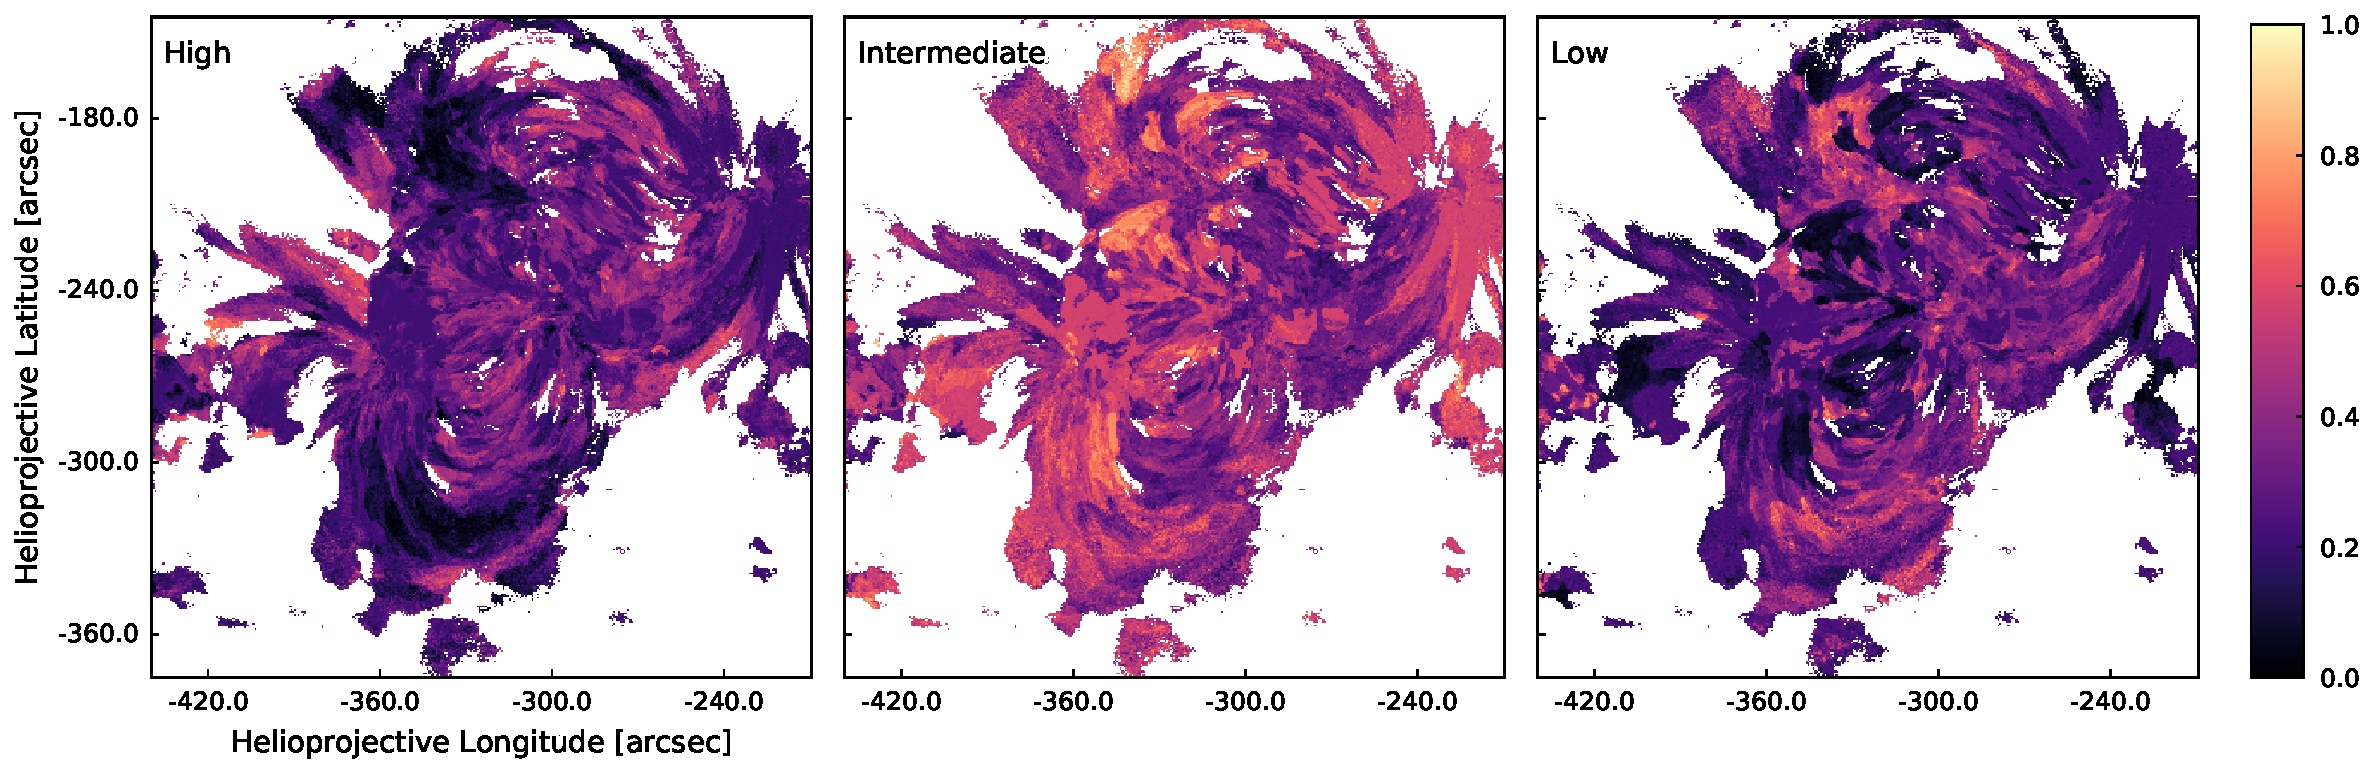
\includegraphics{../figures/class_probability_maps}
        \label{fig:probability_maps}
        \caption{\textbf{Top:} Discrete classification of each observed pixel according to the random forest classifier. \textbf{Bottom:} Class probability of each heating model. The classification of each pixel is determined by the most probable class (i.e. heating model)}
      \end{figure}
      \vspace{-2ex}
    \end{block}
    %
    % em slopes
    %% comparison to emission measure slopes
    \begin{block}{Comparing to Emission Measure Slopes}
      \vspace{-1ex}
      \begin{itemize}
        \item Compute emission measure distribution $\text{EM}(T)$ from time-averaged AIA intensities in each pixel using method of \citet{hannah_differential_2012}
        \item Calculate power law index $a$ such that $\text{EM}\sim T^a$ between 1 and 4 MK
        \item Shallower slope indicates broad distribution of temperatures and thus lower frequency (and \textit{vice versa}) \citep[see][and references therein]{bradshaw_diagnosing_2012,warren_systematic_2012}
        \item Observed range of slopes is broad, \alert{indicating a range of heating frequencies over the active region core}
      \end{itemize}
      \begin{figure}
        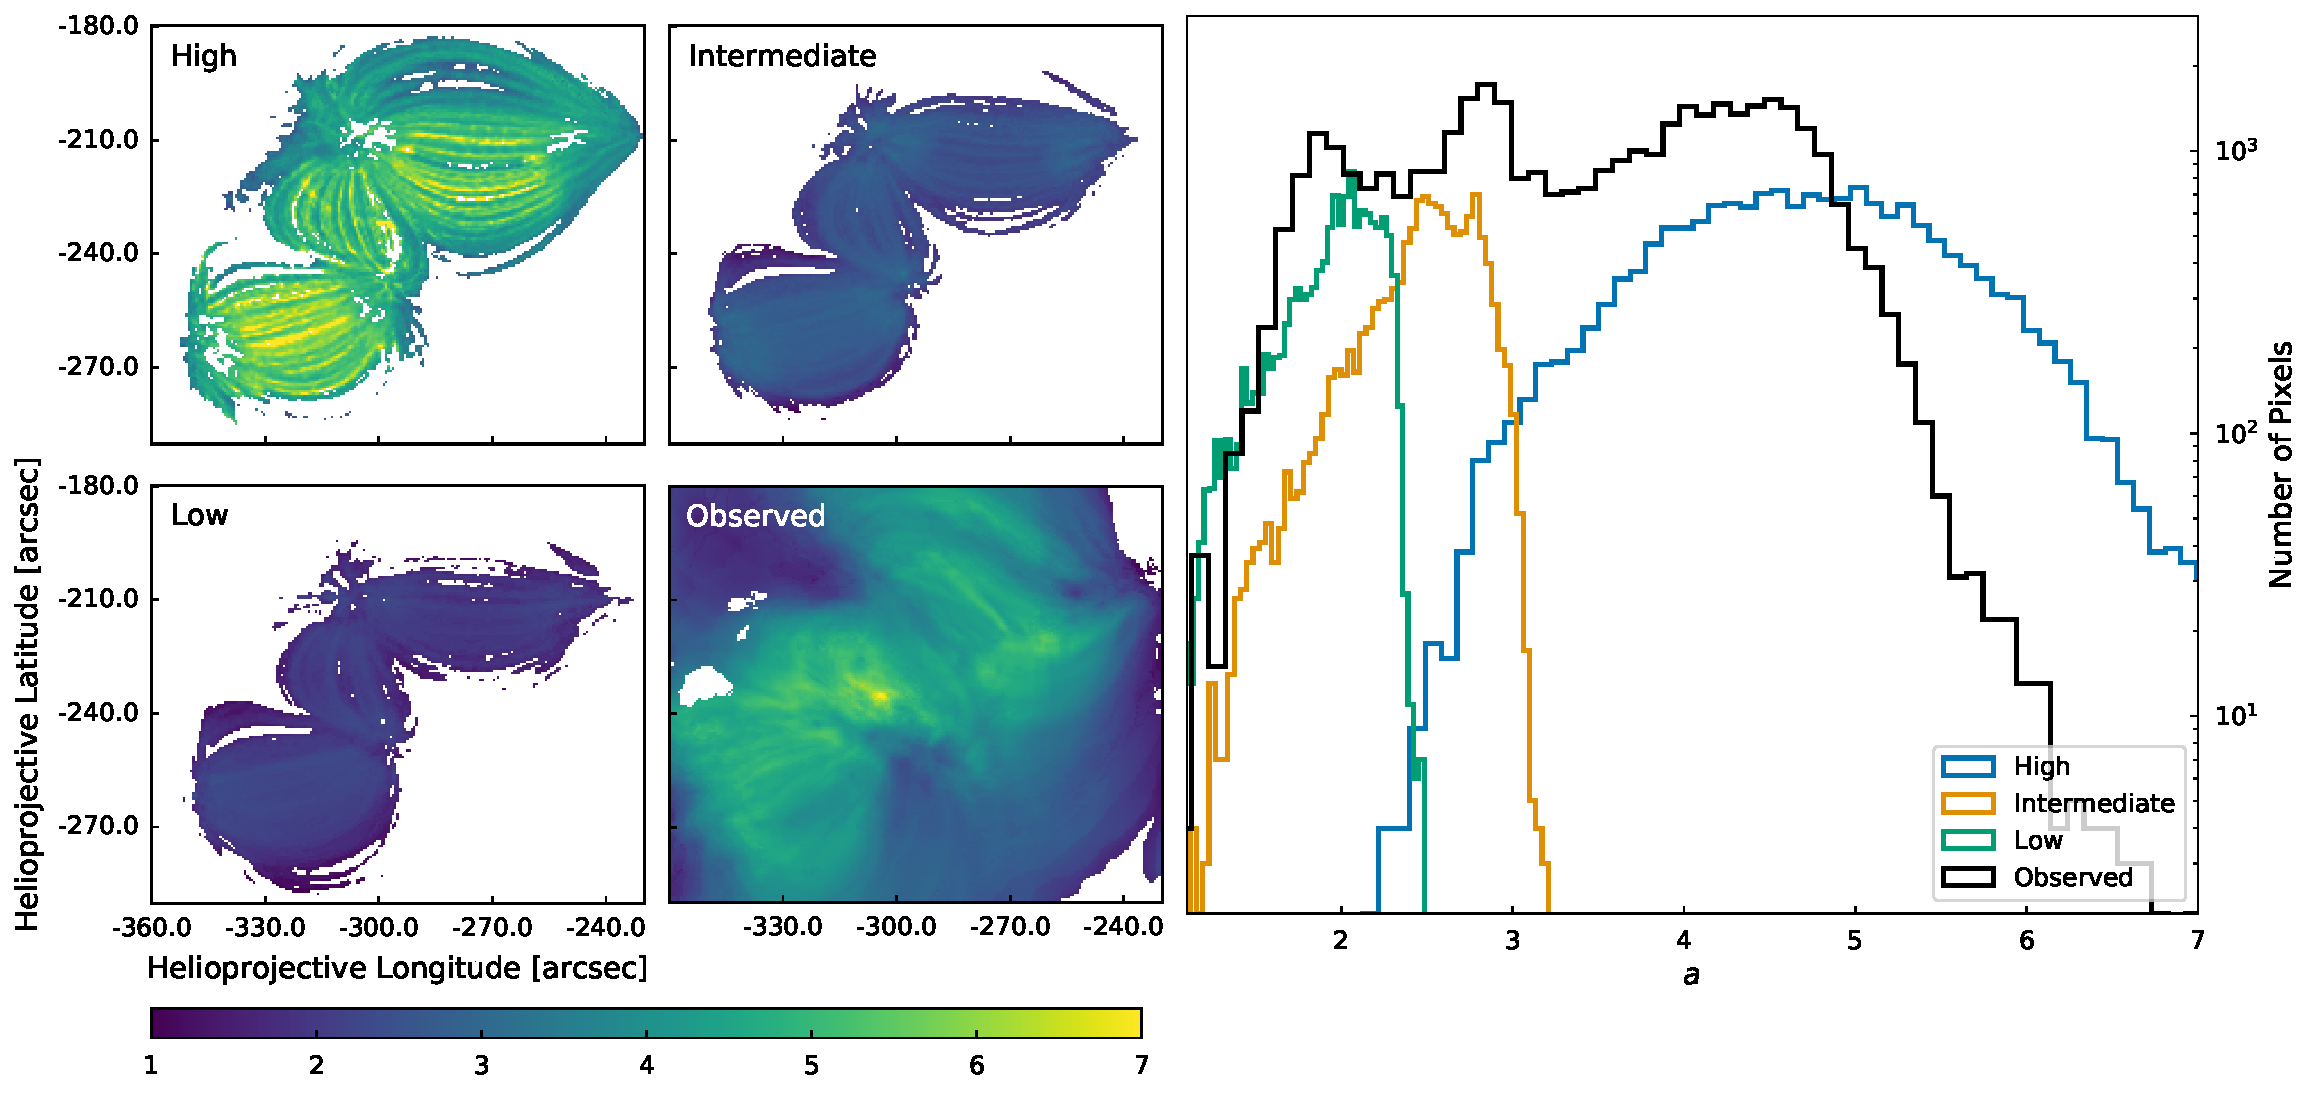
\includegraphics{../figures/em_slopes}
        \label{fig:em_slopes}
        \caption{\textbf{Left:}Emission measure slopes derived from model intensities for three primary heating models and observed intensities. \textbf{Right:} Distribution of emission measure slopes over the active region core.}
      \end{figure}
      \vspace{-2ex}
    \end{block}
    %
    %Conclusions
    \begin{block}{Conclusions}
      \vspace{-1ex}
      \begin{itemize}
        \item Developed flexible, extensible pure Python pipeline for efficiently modeling coronal emission 
        \item Computed timelags suggest \alert{core emission $<10$ MK and heated at sufficiently high frequency}, longer loops on periphery heated at lower frequencies
        \item Application of random forest classifier suggests \alert{dominance of intermediate frequencies over whole AR}
        \item Emission measure slopes show need for \alert{range of heating frequencies} across the AR core
        \item Combination of forward modeling, multiple observables, and classifier approach provide a \alert{powerful method for systematically assessing heating model viability}
      \end{itemize}
    \end{block}
    %
    %references
    \begin{block}{References}
      \scriptsize
      \begin{multicols}{2}
        \bibliographystyle{../../apj.bst}
        \bibliography{references.bib}
      \end{multicols}
    \end{block}
  \end{column}
  \end{columns}
\end{frame}
\end{document}
